\documentclass[tikz,border=2pt]{standalone}
\usepackage{amsmath,amssymb}
\usepackage{tikz}
\usetikzlibrary{arrows.meta}

\begin{document}
% Branch-and-bound tree for max 3x1 + 2x2 s.t. 2x1 + 2x2 <= 9.5, x1 <= 3.5, x integer:
% branch on the fractional x2 of the root relaxation, then on x1; each node carries the
% bound of its LP relaxation.
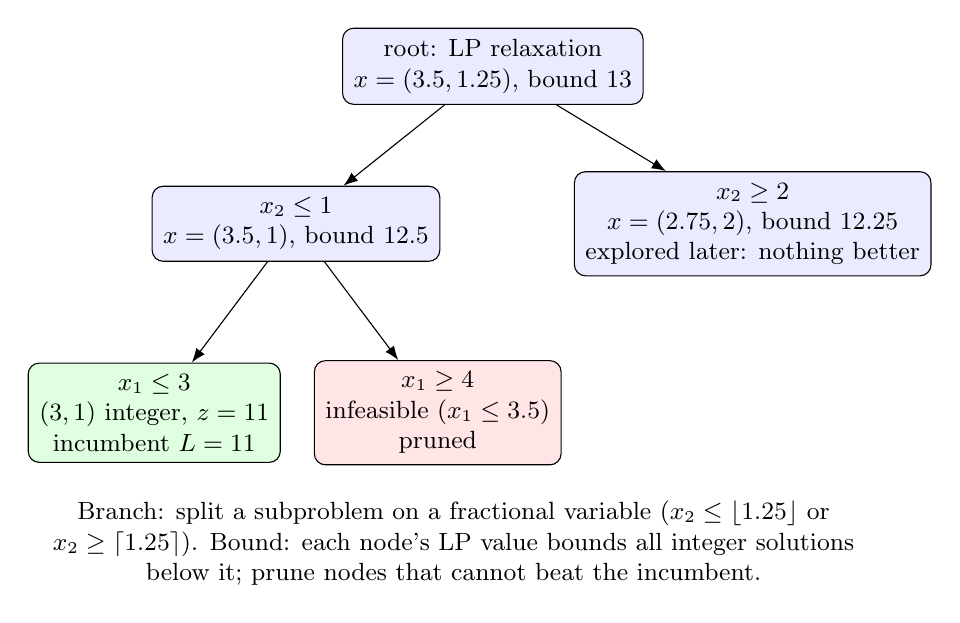
\begin{tikzpicture}[every node/.style={font=\small}, >={Latex[length=1.8mm]}, nd/.style={draw, rounded corners=4pt, fill=blue!8, inner sep=4pt, align=center}]
	\node[nd] (r) at (0,0) {root: LP relaxation\\ $x=(3.5,1.25)$, bound $13$};
	\node[nd] (a) at (-2.5,-2.0) {$x_2\le1$\\ $x=(3.5,1)$, bound $12.5$};
	\node[nd] (b) at (3.3,-2.0) {$x_2\ge2$\\ $x=(2.75,2)$, bound $12.25$\\ explored later: nothing better};
	\node[nd, fill=green!12] (aa) at (-4.3,-4.4) {$x_1\le3$\\ $(3,1)$ integer, $z=11$\\ incumbent $L=11$};
	\node[nd, fill=red!10] (ab) at (-0.7,-4.4) {$x_1\ge4$\\ infeasible ($x_1\le3.5$)\\ pruned};
	\draw[->] (r) -- (a); \draw[->] (r) -- (b);
	\draw[->] (a) -- (aa); \draw[->] (a) -- (ab);
	\node[anchor=north, align=flush center, text width=10.4cm] at (-0.5,-5.4) {Branch: split a subproblem on a fractional variable ($x_2\le\lfloor1.25\rfloor$ or $x_2\ge\lceil1.25\rceil$). Bound: each node's LP value bounds all integer solutions below it; prune nodes that cannot beat the incumbent.};
\end{tikzpicture}
\end{document}
